\documentclass[11pt]{article}
\usepackage[margin=1in]{geometry}
\usepackage[T1]{fontenc}
\usepackage{lmodern}
\usepackage{microtype}
\usepackage{booktabs}
\usepackage{tabularx}
\usepackage{graphicx}
\usepackage{caption}
\usepackage{enumitem}
\usepackage[numbers,sort&compress]{natbib}
\usepackage{xcolor}
\usepackage{placeins}
\usepackage{xurl}
\usepackage{tikz}
\usetikzlibrary{positioning,arrows.meta,fit,backgrounds}
\usepackage[colorlinks=true,linkcolor=blue!50!black,citecolor=blue!50!black,urlcolor=blue!50!black]{hyperref}
\setlist{itemsep=2pt,topsep=4pt}
\captionsetup{font=small,labelfont=bf}
\newcommand{\forum}[1]{\href{https://www.kaggle.com/competitions/gemma-4-developer-agent/discussion/#1}{forum #1}}
\newcommand{\tool}[1]{\texttt{\detokenize{#1}}}
\definecolor{kitblue}{HTML}{2A78D6}
\definecolor{kitorange}{HTML}{EB6834}
\definecolor{kitgrey}{HTML}{52514E}

\title{\textbf{Scorer in a Box: A One-GPU Replica of the Gemma 4 Agent Scorer, and the Silent Failures It Catches}\\[8pt]
\large An open kit for evaluating, debugging and fine-tuning local coding agents under the competition's real conditions}
\author{Shashanka B R\\\small\texttt{shashanka.b.r@ibm.com}\\[4pt]\small Gemma 4 Developer Agent Paper Track, Best New Resource\\\small Code: \url{https://github.com/shashanka300/runtime-bound}}
\date{November 2026}

\begin{document}
\maketitle

\begin{abstract}
A fine-tuned adapter that changed nothing. A thinking budget that never reached the model. An engine that quietly removed the agent's own earlier reasoning from every prompt. None of these were bugs in our agent: they were in the competition's scoring stack, and none of them raised an error. Each one showed up only as a few points of score, through a feedback loop of one submission a day, a day of queueing and a single number back, where a broken stack and a bad idea look exactly the same. Scorer in a Box is an open kit that makes such failures visible on one consumer GPU. It serves the scorer's exact engine build and flags, runs the official harness at the scorer's speed, compiles every bundle with the scorer's own code before it spends a submission, and adds probes for the parts of the stack that fail quietly: a random-weight adapter canary, a cross-check of sampling settings against the scorer's own translation code, and a proxy that replays identical multi-turn requests on two engines. In seven weeks it caught six silent failures: the three above, all later confirmed or fixed by the organizers; two in our own setup that had looked exactly like experimental results, including a 12.5-point ``engine effect'' that turned out to be a dropped configuration flag; and a released test environment that can grade only 41 of the 129 public tasks. The kit also provides per-turn trace analysis, 142 competition-format tasks from 116 repositories outside the public set, and a LoRA trainer for the competition's packed int4 checkpoint, which standard tooling cannot fine-tune. Each component is described with the failure it exists to catch, and all of it is open source.
\end{abstract}

\section{Introduction}
Agent competitions evaluate a whole stack, not a model: a serving engine, a chat template, an agent framework, a sandbox, a dependency set and a clock. In the Gemma~4 Developer Agent competition~\citep{gemma4paper2026} that stack runs on 4$\times$L4 GPUs behind a submission queue. Participants see a public development set of 129 tasks and a leaderboard number per day.

That combination makes silent failures expensive. A wiped adapter, an ignored parameter or a broken test environment does not raise an error; it changes the score by a few points, and a few points is inside the board's noise. Our first submission solved 31\% of tasks locally and scored 0.03 on the board; the companion paper~\citep{runtimebound2026} traces that gap. This paper describes the tooling that made the trace possible, released as a resource.

The kit is built around one rule: \emph{when local and scorer can differ, run the scorer's own code}. Where we could not run it, we built a probe that tells the two apart. Table~\ref{tab:caught} lists what that caught.

\begin{table}[!htb]
\centering\footnotesize
\begin{tabularx}{\linewidth}{>{\raggedright\arraybackslash}p{2.9cm}X>{\raggedright\arraybackslash}p{3.0cm}}
\toprule
Component & Silent failure it caught & Outcome \\
\midrule
LoRA canary & The scorer's vLLM build wiped adapter weights: a random-weight canary gave output identical to the base model. & Fixed by the organizers. \\
Thinking cross-check & The harness validated \tool{thinking_budget} but never sent it to the engine. & Fixed (\forum{744566}). \\
Record + replay proxy & vLLM 0.19.1 dropped the agent's earlier \tool{reasoning_content} from the prompt (418 tokens shorter at turns 2--4, 2,583 from turn 5). & Fixed; independently reported (\forum{744354}). \\
Serving-flag audit & vLLM's YAML loader silently drops boolean \texttt{false}; a KV-reservation flag was never applied, causing stalls we first read as a 12.5-point engine effect. & Local; flag now passed on the command line. \\
Per-pool wheel cache & The harness caches unpacked wheels under one fixed name; a cache from another wheel pool broke pytest on every task of a screen (0/19). & Local fix; reported (\forum{744029}). \\
Gold-patch sweep & Only 41 of 129 public tasks can be graded offline with the released environment. & Reported; hidden set validated at 100\% by the organizers. \\
\bottomrule
\end{tabularx}
\caption{Six silent failures and the component that caught each. None of them raised an error.}
\label{tab:caught}
\end{table}

\section{The kit}
Figure~\ref{fig:kit} shows how the parts connect. Everything runs on one RTX 5090 (32\,GB) under WSL2; the LoRA trainer also runs on a rented H100.

\begin{figure}[!htb]
\centering
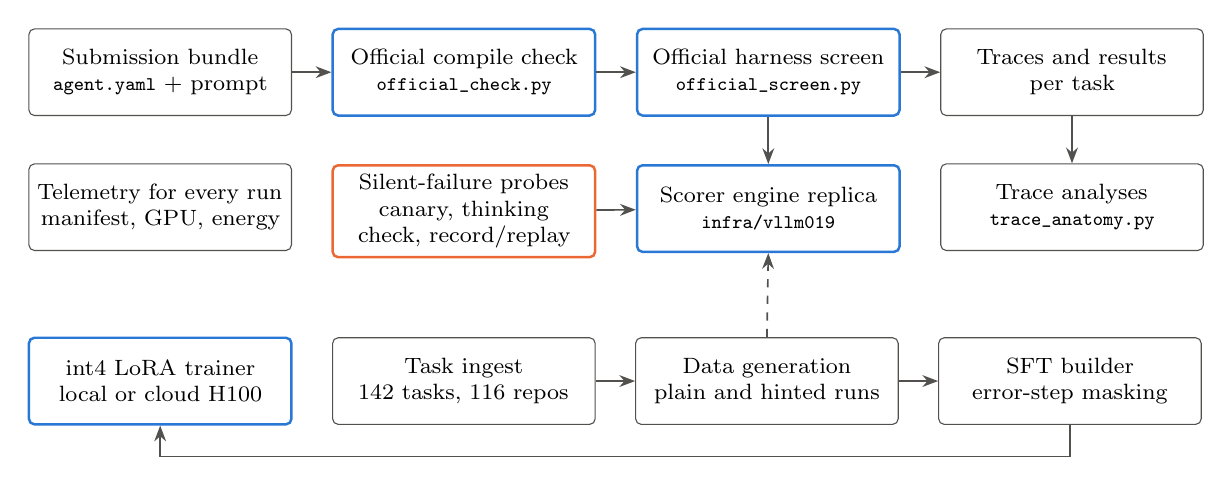
\begin{tikzpicture}[
  node distance=6mm and 5mm,
  box/.style={draw=kitgrey, rounded corners=2pt, align=center, font=\footnotesize, minimum height=11mm, text width=31mm, fill=white,
              execute at begin node={\hyphenpenalty=10000\exhyphenpenalty=10000}},
  core/.style={box, draw=kitblue, line width=0.9pt},
  probe/.style={box, draw=kitorange, line width=0.9pt},
  arr/.style={-{Stealth[length=2mm]}, kitgrey, line width=0.6pt},
  p/.style={font=\scriptsize\ttfamily}
]
\newcommand{\fn}[1]{{\scriptsize\texttt{\detokenize{#1}}}}
\node[box] (bundle) {Submission bundle\\\fn{agent.yaml} + prompt};
\node[core, right=of bundle] (check) {Official compile check\\\fn{official_check.py}};
\node[core, right=of check] (screen) {Official harness screen\\\fn{official_screen.py}};
\node[box, right=of screen] (traces) {Traces and results\\per task};
\node[probe, below=of check] (probes) {Silent-failure probes\\canary, thinking check, record/replay};
\node[core, below=of screen] (vllm) {Scorer engine replica\\\fn{infra/vllm019}};
\node[box, below=of traces] (analysis) {Trace analyses\\\fn{trace_anatomy.py}};
\node[box, below=of bundle] (tele) {Telemetry for every run\\manifest, GPU, energy};
\node[box, below=10mm of probes] (ingest) {Task ingest\\142 tasks, 116 repos};
\node[box, right=of ingest] (gen) {Data generation\\plain and hinted runs};
\node[box, right=of gen] (sft) {SFT builder\\error-step masking};
\node[core, left=of ingest] (qlora) {int4 LoRA trainer\\local or cloud H100};
\draw[arr] (bundle) -- (check);
\draw[arr] (check) -- (screen);
\draw[arr] (screen) -- (traces);
\draw[arr] (traces) -- (analysis);
\draw[arr] (screen) -- (vllm);
\draw[arr] (probes) -- (vllm);
\draw[arr] (ingest) -- (gen);
\draw[arr] (gen) -- (sft);
\draw[arr] (sft.south) -- ++(0,-4mm) -| (qlora.south);
\draw[arr, dashed] (gen.north) -- (vllm.south);
\end{tikzpicture}
\caption{The kit. Blue: parts that run the scorer's own code or reproduce its configuration. Orange: probes that detect where local and scorer behaviour silently diverge. The training path (bottom) reuses the same engine and harness to generate data.}
\label{fig:kit}
\end{figure}

\subsection{Scorer engine replica}
\tool{infra/vllm019/} installs the scorer's vLLM~0.19.1~\citep{kwon2023vllm} and every serving dependency from the organizers' wheelhouse with \texttt{--no-deps} at the pinned versions, so a resolver cannot pull a newer transformers (it did, once). It serves with the scorer's flags and passes boolean flags on the command line, because the YAML config path drops \texttt{false}. A 12B profile adds the architecture override the organizers published for that checkpoint.

\subsection{Official harness screen}
\tool{tools/official_screen.py} evaluates a bundle with the official harness (swegemma, adk\_submission, google-adk at the wheelhouse versions), configured like the organizers' getting-started notebook, against the local engine. Two choices make its numbers comparable to the scorer: tasks run one at a time, as on the scorer, and the per-task time cap is scaled by 0.625 because the L4 box decodes about 1.6$\times$ slower. It gives each wheel pool its own temporary directory, since the harness's wheel cache is keyed by a fixed name. \tool{tools/overnight_screen.sh} wraps it with engine start-up, a health watchdog and resumable rows.

\subsection{Compile check before submitting}
\tool{leaderboard/official_check.py} validates and compiles a bundle with the scorer's own submission code and the real tool signatures, without calling a model. With one submission per day and a day-long queue, a packaging error costs a day, so we run it on every bundle before submitting. \tool{leaderboard/build.py} generates every bundle from code, so each submitted file has a recorded derivation.

\subsection{Silent-failure probes}
\begin{itemize}
\item \textbf{LoRA canary} (\tool{tools/lora_canary*.py}) copies an adapter's layout, fills \texttt{lora\_B} with random values and compares greedy output and top-5 log-probabilities against the base model. An applied adapter must change them; on the original scorer build it did not, on the patched build the canary's log-probability moved from $-13.125$ to $-12.19$. An all-linear variant also measures the decode cost of an adapter (66.9 to 57.4 tokens/s, $-14\%$, for rank 16 on all linear layers).
\item \textbf{Thinking cross-check} (\tool{tools/check_official_thinking.py}) runs a grid of sampling configs through the scorer's own translation function and exits non-zero if the local harness would send anything different. It is meant to run after every wheelhouse update.
\item \textbf{Record and replay} (\tool{tools/record_proxy.py}, \tool{tools/replay_requests.py}) is a transparent proxy that records every chat request of a real agent session, and a replayer that sends the identical requests to another engine. Because inputs are fixed, any difference in prompt length or output is the engine's rendering of history, not the agent.
\end{itemize}

\subsection{Gradability audit}
\tool{tools/official_gold_sweep.py} applies each task's reference patch and runs its tests through the official air-gapped verification path. It found that only 41 of 129 public tasks are gradable offline with the released environment (rich 39/48, httpx 1/1, fastapi 1/67, requests 0/13), with the causes per task (missing test packages, SSL failures on Python 3.13, installed packages shadowing the workspace). The result, \tool{leaderboard/official_gradability.csv}, is the task list every screen uses. Our own harness, swebox, fills missing packages at image build and grades 114 of 129; \tool{tools/regrade_swebox.py} uses it to grade runs the official grader cannot (it matched the official grader on 4 of 4 overlapping patches).

\subsection{Trace analyses}
\tool{tools/trace_anatomy.py} turns a screen's traces into a per-task anatomy: turns, output tokens, the longest turn, the share of time in the three slowest turns, time to the first edit, and repetition loops (turns where more than a quarter of the sentences repeat). It produced the finding that timed-out tasks lose 62\% of their time in one to three turns at the thinking cap~\citep{runtimebound2026}. \tool{tools/behaviour_scan.py} classifies every tool call (duplicate, overlapping re-read, repeated search, error, retry) to measure wasted calls.

\subsection{Telemetry}
Every run writes a manifest (git state, config hash, package and lockfile hashes, GPU, driver, engine version, served model, data fingerprint), structured logs, spans, 1\,Hz NVML samples with the energy counter, container resource use and the engine's Prometheus counters. \tool{rbcore.windows} attributes any of them to a task or phase, for example energy per task. \tool{tools/otel_bridge.py} forwards training and cost metrics to any OTLP dashboard; we used it to watch a cloud training run against a credit cap. The KV-reservation artefact in Table~\ref{tab:caught} was found in this telemetry, as requests waiting with an empty KV cache.

\subsection{Multi-repository tasks}
The public set covers four repositories, and the hidden set others. \tool{tools/ingest_rebench.py} converts SWE-rebench~\citep{badertdinov2025swerebench} tasks into the competition's on-disk format: task records, a snapshot of each repository at its base commit, Python~3.13 wheels for its dependencies, and empty graph and embedding folders. A self-check keeps only tasks whose reference patch passes and whose empty patch fails. From 319 snapshotted tasks it kept \textbf{142 tasks from 116 repositories}; the 175 rejects are recorded with their failure class (collection errors 133, failing tests 41). Because the format matches, the official harness and every tool above run on them unchanged. We release the script, not the data; the source dataset is CC-BY-4.0.

\subsection{Fine-tuning the int4 checkpoint}
The competition's 31B checkpoint stores its linear layers in a packed int4 format (compressed-tensors, group size 32) that standard PEFT tooling cannot wrap. \tool{tools/qlora.py} replaces each of the 410 packed layers with a module that unpacks its weight to bf16 inside forward and backward (bit-exact against the reference unpacker, nothing saved for backward) and adds LoRA~\citep{hu2022lora,dettmers2023qlora}. \tool{tools/train_lora.py} trains on overlapping 8k-token windows with gradient checkpointing, keeps the optimizer and master weights on the CPU so a 32\,GB card fits rank 16 on all linear layers (122.4M parameters), masks the loss on tool calls that failed as calls, holds out validation runs, and saves resumable state every ten steps. \tool{tools/build_sft.py} builds the training set from solved runs, including hinted runs with the hint redacted. \tool{tools/modal_train.py} runs the same trainer on a cloud H100 as a detached job that survives a dropped client, with a credit guard. The two machines produced the same initial loss, validation loss and first-step loss (0.2452, 0.3829, 0.3915), so cloud and local runs are interchangeable.

\section{Using the kit}
A typical loop for a new agent idea is: build the bundle with \tool{leaderboard/build.py}; check it with \tool{official_check.py}; screen it with \tool{overnight_screen.sh} on the 39 gradable tasks (about three hours) or on a multi-repository task root via \texttt{COMP\_DIR}; compare it paired against the baseline; and read \tool{trace_anatomy.py} before reading the score, because the score alone does not say why. Before trusting any result that involves adapters, sampling or a new wheelhouse, run the canary and the thinking cross-check. The repository README maps each result in the companion paper to the code and records that produced it.

\section{Related work}
SWE-bench~\citep{jimenez2024swebench} and its harness define the task and grading format the competition follows; SWE-agent~\citep{yang2024sweagent} showed how much the agent--computer interface matters for a fixed model, which is why we test interfaces against the scorer's own. SWE-rebench~\citep{badertdinov2025swerebench} provides continuously collected, decontaminated tasks; our ingest makes them runnable in this competition's environment. SWE-Gym~\citep{pan2025swegym} provides executable environments for training agents; our trainer targets the one quantized checkpoint a competitor must use. Paired, interval-based reporting follows~\citet{agarwal2021rliable}.

\section{Limitations}
The replica is faithful to the scorer's code, not to its hidden tasks: local solve rates were 3--10$\times$ the leaderboard, because the hidden repositories differ from the public ones. The 0.625 time scaling models decode speed only, not prefill. The multi-repository task set has not been validated as a predictor of the leaderboard. The kit targets this competition's stack (vLLM 0.19.1, ADK, swegemma); the probes are general ideas, but their code assumes these interfaces. Several components depend on files only available after accepting the competition rules, which we do not redistribute.

\section{Availability}
Code, configuration and run summaries: \url{https://github.com/shashanka300/runtime-bound} (MIT; third-party files listed in \texttt{NOTICE}). Every deviation from our pre-registered plan, with the evidence available at the time, is in \nolinkurl{docs/design_changes.md}.

\bibliographystyle{plainnat}
\bibliography{refs}
\end{document}
